\documentclass[12pt,letterpaper]{report}
\usepackage{graphicx}
\graphicspath{{Imagenes/}}
\usepackage[utf8]{inputenc}
\usepackage[spanish]{babel}
\usepackage[utf8]{inputenc}
\usepackage{multicol}
\usepackage[left=2cm,right=2cm,top=2cm,bottom=2cm]{geometry}
\setlength{\parindent}{0 pt}
\pagestyle{empty}
\pagenumbering{arial}
\author{Mark Brian Paredes Zavala}
\title{Proyecto Final}

\begin{document}

\maketitle

\begin{center}
Procesador de Textos.
\end{center}
Este proyecto fue realizado en el lenguaje de C en el compilador de (DEV-C++)\\ 
El programa es un procesador de textos, mediante un archivo .txt que le llamaremos (ArchivoEntrada) y mediante una serie de comandos escritos, que realizaran una determinada acción, las cuales son:\\ 

\begin{enumerate}
\item L\_ d1\_ d2 \_ dn: Atributo de la linea L imprimirá solamente las lineas indicadas por d1\_ d2 \_ dn... etc donde \_ es el separador de dígitos. 
\item C\_ d1\_ d2\_ dn: Atributo columna imprimirá solamente las columnas indicadas por d1\_ d2 \_ dn... etc donde \_ es el separador de digitos.
\item ILV\_ d1\_ d2\_ dn: El atributo intercalar meterá un salto de linea en  las lineas indicadas por d1\_ d2 \_ dn... etc donde \_ es el separador de digitos.
\item IC\_ d1\_ d2\_ dn: El atributo Intercalar columnas IC meterá un tabulador solamente en las lineas indicadas por d1\_ d2 \_ dn... etc donde \_ es el separador de dígitos
\item CC (cadena) : Contador de cadenas, contar únicamente el numero de ocurrencias en cada cadena encontrada indicando el numero de ocurrencias en cada linea:
\item CP (cadena): El atributo contador de prefijos contara únicamente el numero de ocurrencias de la subcadena dada que sea prefijo de cada cadena del archivo, indicando el numero de ocurrencias de cada linea.
\item CS (cadena): El atributo contador de sufijos contara únicamente el numero de ocurrencias de la subcadena dada que sea sufijo de cada cadena del archivo, indicando el numero de ocurrencias de cada linea.
\item WC: Cuenta cadenas, caracteres y numero de lineas.
\item WNUM: Cuenta el numero de ocurrencia de enteros y flotantes.
\item INC: Insertara el numero de fila, numerando cada linea del archivo.
\end{enumerate}
\newpage
En consola realizaremos la ejecución del programa mediante la siguiente sintaxis:\\\\

\textbf{\textit{ ''Programa Ejecutable.exe''  ''ArchivoEntrada.txt''  ''Atributo''  ''ArchivoSalida.txt'' }}\\

\begin{center}
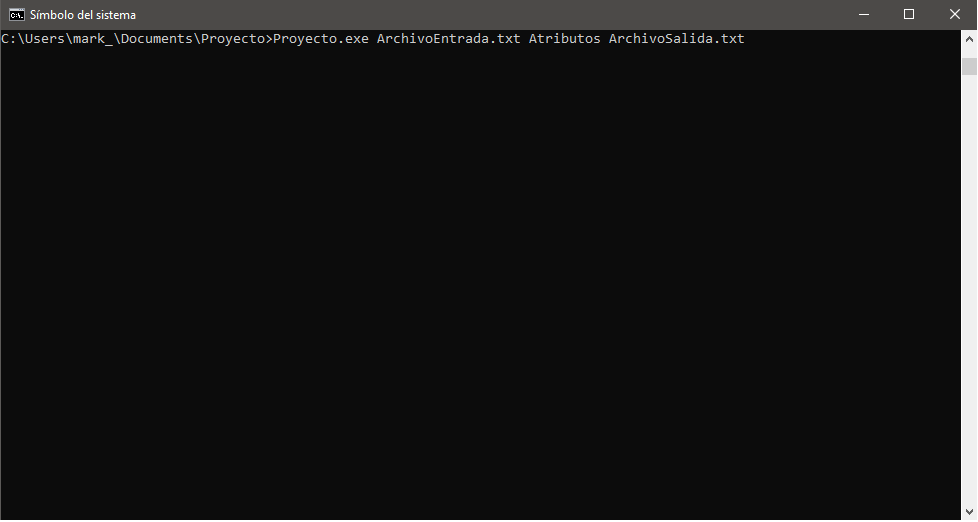
\includegraphics[scale=0.5]{Sintaxis}
\end{center}
Así es como se vería el ingreso de la sintaxis en el cmd mejor conocido como ''Símbolo del sistema''. \\
Antes tenemos que especificar al cmd la ruta donde tenemos nuestros archivos que utlizaremos para este programa\\
Primero tendremos que buscar el cmd en nuestro ordenador:\\

\begin{center}
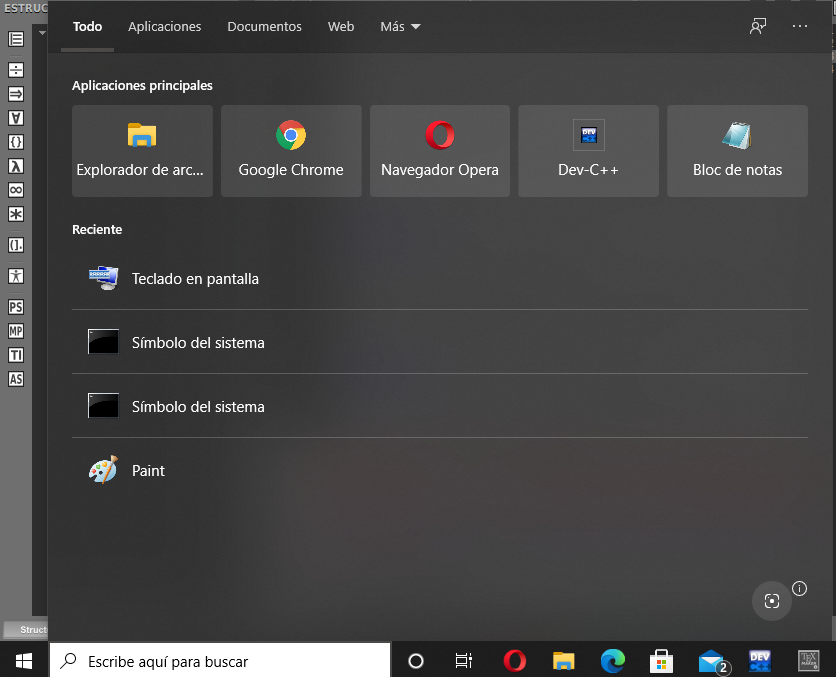
\includegraphics[scale=0.35]{ruta01}
\end{center}

En mi caso ya lo tengo por predeterminado en mi inicio por lo que ingresare.\\
Cuando hayamos ingresado se nos abrirá el cmd de esta forma:

\begin{center}
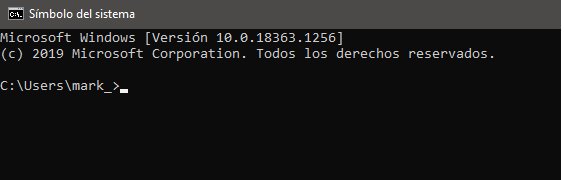
\includegraphics[scale=0.5]{ruta1}
\end{center}

Dentro de cmd tendremos que especificar la ruta de donde tenemos nuestro proyecto:

\begin{multicols}{2}
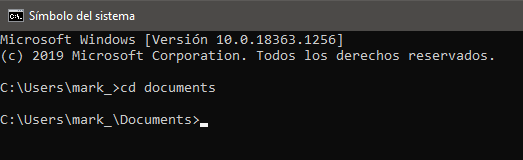
\includegraphics[scale=0.5]{ruta2}
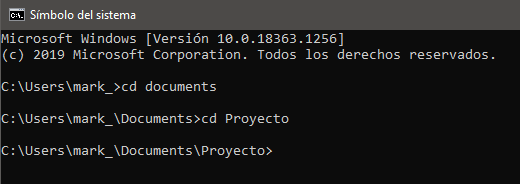
\includegraphics[scale=0.5]{ruta3}
\end{multicols}

De esta forma tendremos acceso a los archivos a utilizar, de igual forma, ejecutar nuestro programa desde cmd donde recibirá argumentos que vamos a menciona mas adelante.

\begin{center}
Ejecución del programa
\end{center}

De acuerdo a las acciones de los atributos y el hecho de ejecutar el programa en cmd se diseño un algoritmo donde resolveremos las situaciones mencionadas anteriormente.\\

En primer lugar tendremos en cuenta que se recibirán argumentos asi que, vamos a definir ¿Comó vamos a pasar comando desde cmd? \\
Cuando queramos recibir comandos tendremos que ejecutar en nuestro int main() con argumentos donde serán los siguientes:\\

\begin{center}
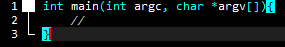
\includegraphics[scale=0.7]{argumentos}
\end{center}

El argc (argument cout) es considerado el numero de argumentos por lo que se ingresa como argumento del main como int, argv (argument vertos) es una array de vectores que va contener los elementos de argc\\

Vamos a considerar como argv[0] como el programa ejecutable, entonces si se ingresa un total de tres argumentos, el valor de argc sera de 4 puesto y argv[0] tendrá como contenido el programa ejecutable (.exe)\\

Entonces, al tener el concepto de recibir argumentos por medio de cmd procedemos a realizar el algoritmo que seria idéntico a la ultima imagen mostrada.\\

De la misma manera, procedemos a deducir el algoritmo para identificar por medio de la linea de argumentos que atributo se eligio, en este programa al recibir 4 argumentos tendremos algo asi:\\\\

\textbf{\textit{ ''argv[0]''  ''argv[1]''  ''argv[2]''  ''argv[3]'' }}\\\\

Esta sintaxis la utilizaremos de los ejemplos 1 al 4 asi como del 8 al 10.\\
Caso contrario, cuando vayamos a ingresar los atributos del ejemplo 5 al 7 donde ingresaremos un argumento de mas:\\

\textbf{\textit{ ''argv[0]''  ''argv[1]''  ''argv[2]''  ''argv[3]''  ''argv[4]'' }}\\

\newpage
A continuación se mostraran la ejecución final del programa:\\

\begin{multicols}{2}
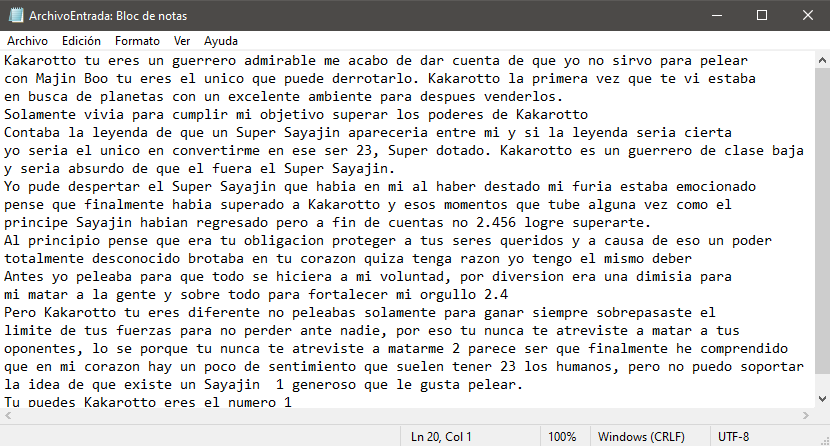
\includegraphics[scale=0.35]{ArchivoEntrada}\\
Podemos observar el texto contenido en el archivo se conocerá como ''Archivo de entrada'', el cual ocuparemos para todo el proyecto, no sera modificando con la ejecución de cada comando, si no el modificado sera el ''Archivo de Salida''.
\end{multicols}


\begin{multicols}{2}
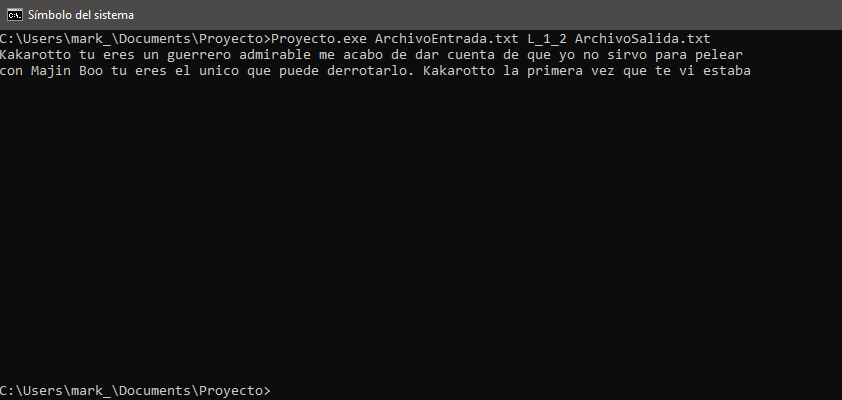
\includegraphics[scale=0.35]{Salida1}
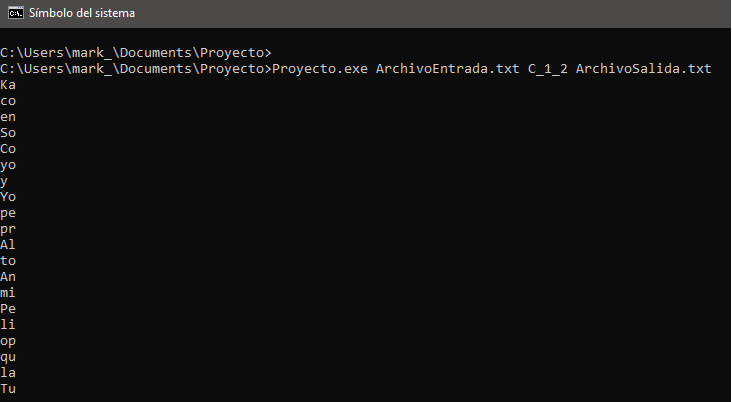
\includegraphics[scale=0.35]{Salida2}
\end{multicols}


\begin{multicols}{2}
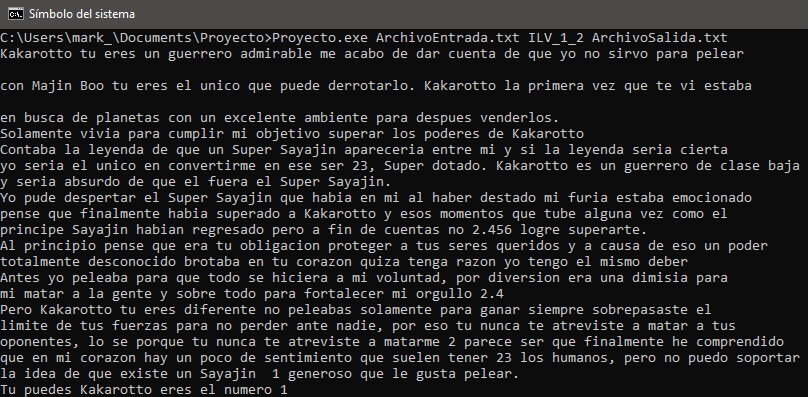
\includegraphics[scale=0.35]{Salida3}
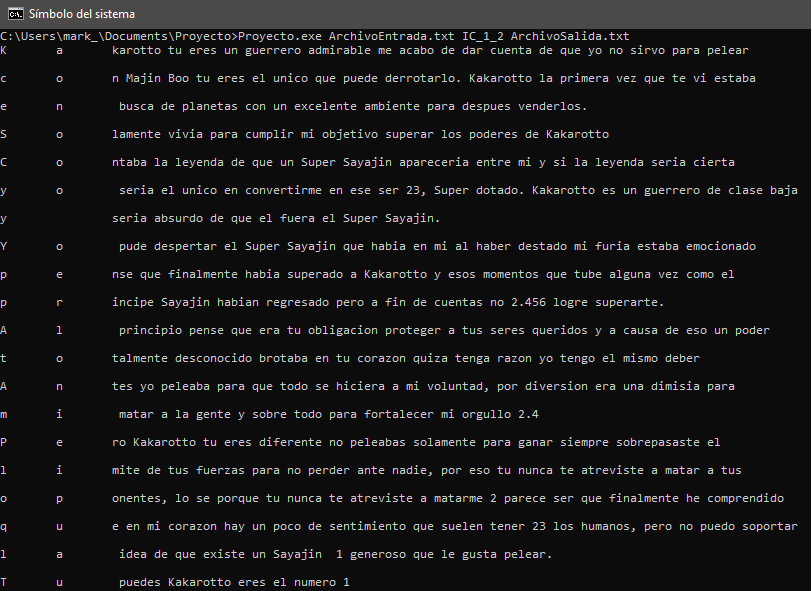
\includegraphics[scale=0.35]{Salida4}
\end{multicols}


\begin{multicols}{2}
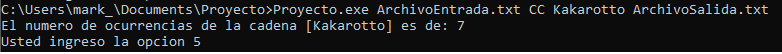
\includegraphics[scale=0.35]{Salida5}\\
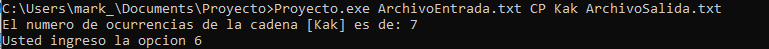
\includegraphics[scale=0.35]{Salida6}
\end{multicols}


\begin{multicols}{2}
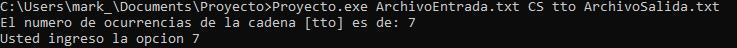
\includegraphics[scale=0.25]{Salida7}\\
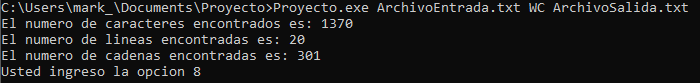
\includegraphics[scale=0.25]{Salida8}
\end{multicols}


\begin{multicols}{2}
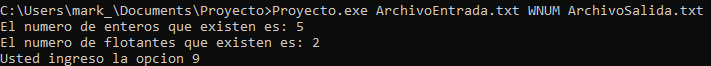
\includegraphics[scale=0.35]{Salida9}\\
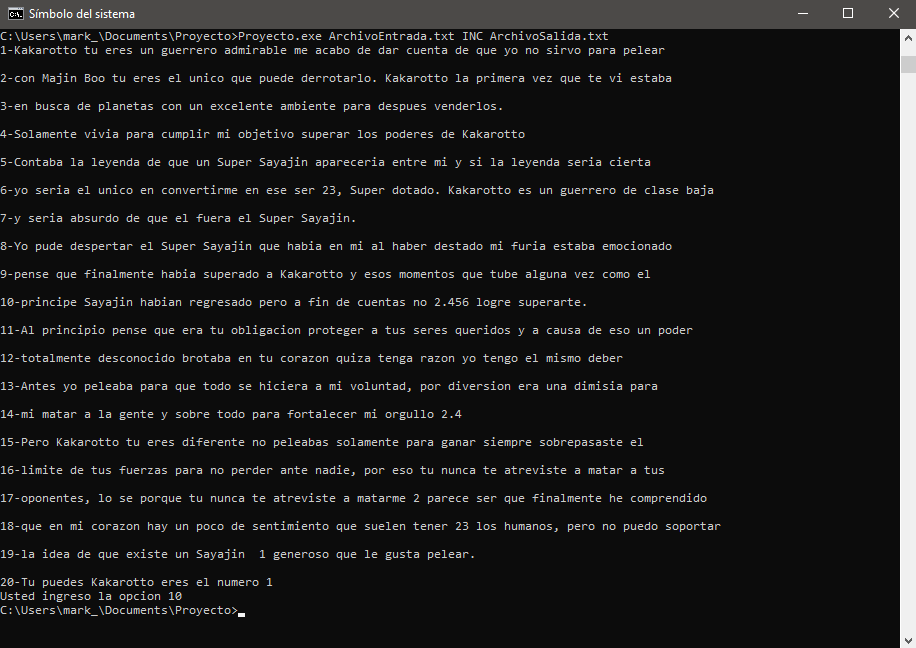
\includegraphics[scale=0.35]{Salida10}
\end{multicols}

\newpage
Ahora se mostrara la lo que se escribió en el ArchivoSalida de acuerdo a cada ejecución:\\

\begin{multicols}{2}
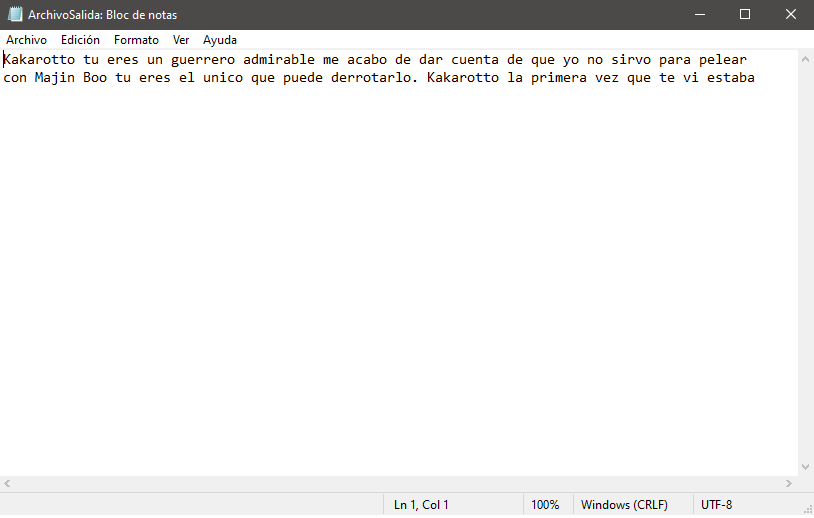
\includegraphics[scale=0.35]{ArchivoSalida1}
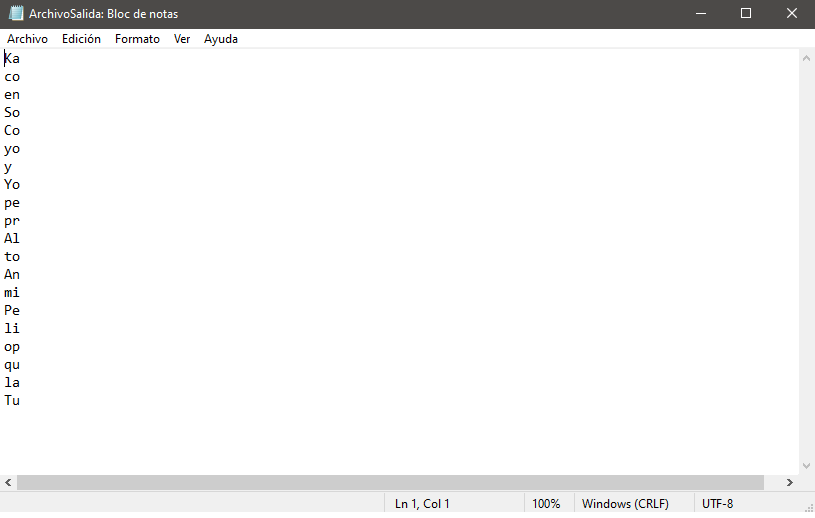
\includegraphics[scale=0.35]{ArchivoSalida2}
\end{multicols}


\begin{multicols}{2}
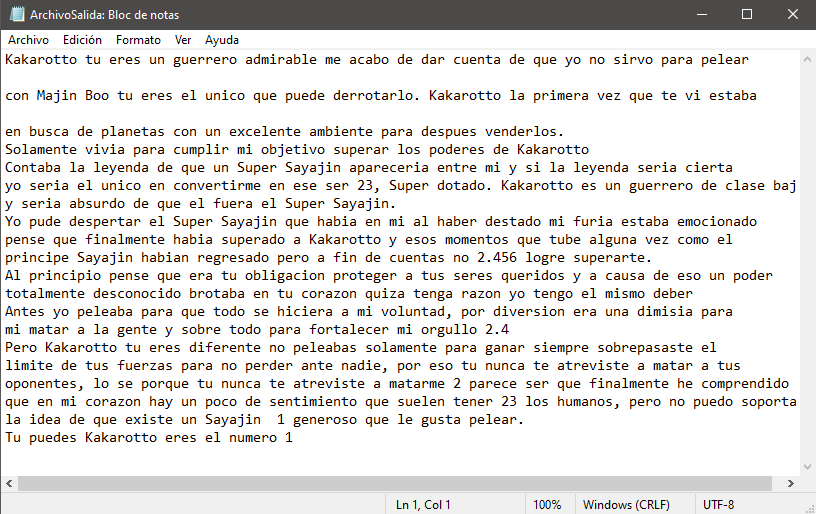
\includegraphics[scale=0.35]{ArchivoSalida3}
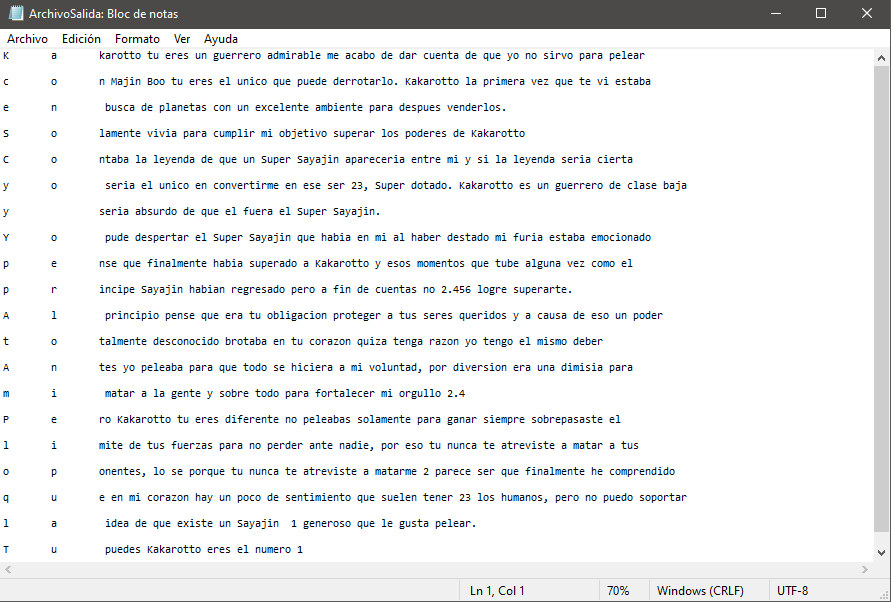
\includegraphics[scale=0.35]{ArchivoSalida4}
\end{multicols}


\begin{multicols}{2}
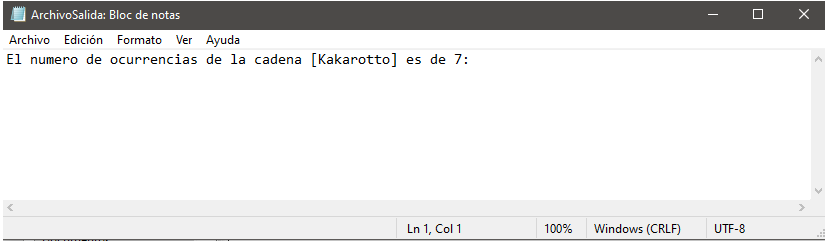
\includegraphics[scale=0.35]{ArchivoSalida5}\\
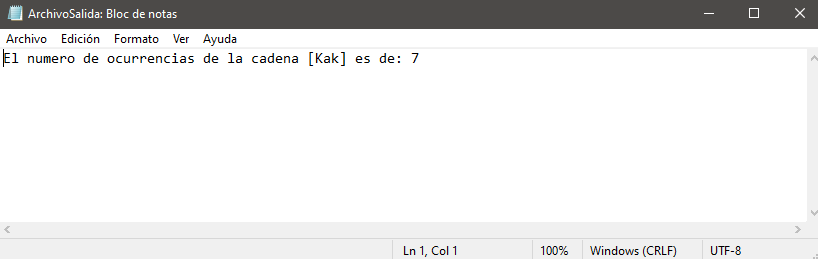
\includegraphics[scale=0.35]{ArchivoSalida6}
\end{multicols}


\begin{multicols}{2}
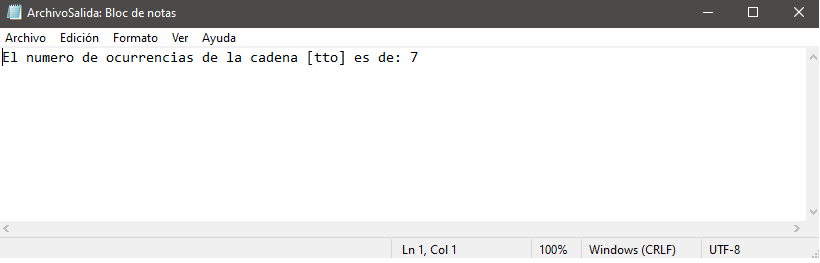
\includegraphics[scale=0.25]{ArchivoSalida7}\\
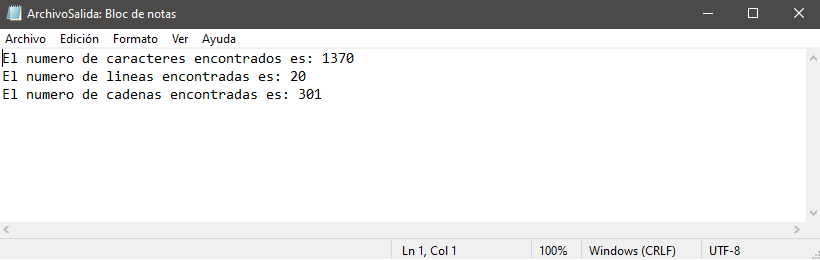
\includegraphics[scale=0.25]{ArchivoSalida8}
\end{multicols}


\begin{multicols}{2}
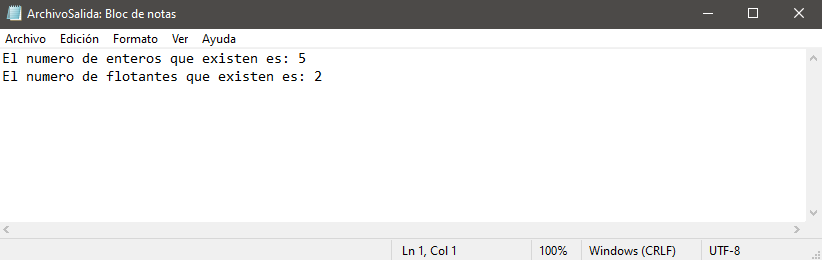
\includegraphics[scale=0.35]{ArchivoSalida9}\\
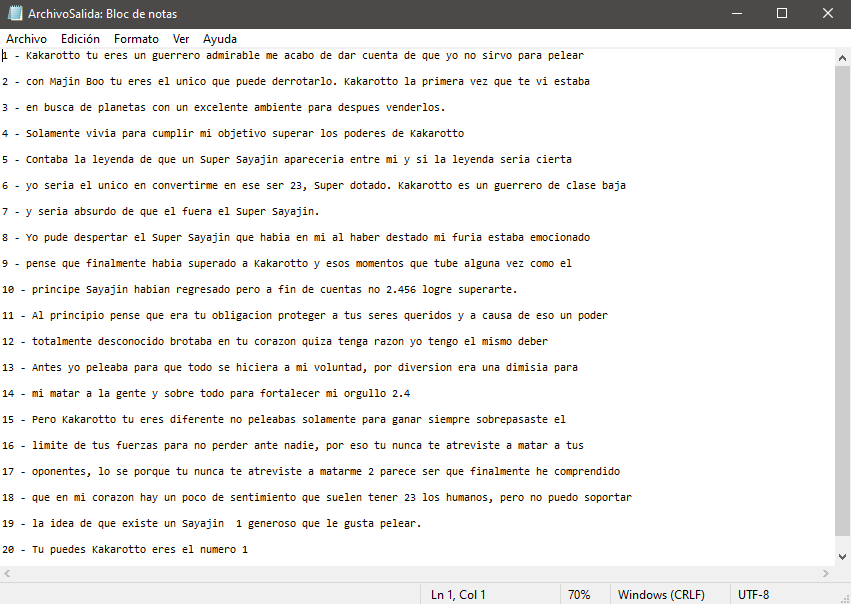
\includegraphics[scale=0.35]{ArchivoSalida10}
\end{multicols}
Como se pudo observar el funcionamiento de código fue de manera correcta, así mismo la salida de la información hacia el Archivo de salida.\\

\begin{center}
Bibliotecas y funciones a utilizar en este programa.\\
\end{center}
A continuacion se muestran las funciones usadas para realizar este proyecto, mediante las cuales se adentrara en especifico a lo que aportaran a este programa:\\

\textbf{\textit{Bibliotecas}}\\


\begin{enumerate}

\item \# include $<$stdio.h$>$: Nos permite manipular con funciones las cuales podremos manipular  asi como el manejo de archivos:\\

\textbf{\textit{Entrada y salida de funciones}}
\begin{enumerate}

\item fopen: Abre un archivo, en el archivo se especifica si se leera, modificara, leer y modificar, etc.
\item fclose: Cierra un archivo con el valor asociado.

\end{enumerate}

\textbf{\textit{\em{Manejo de archivos}}}

\begin{enumerate}
\item feof: Comprueba si al final de un archivo pasa determinado flujo
\item fgets: obtiene una cadena desde el archivo y termina en una nueva linea o al final de archivo.
\item fgetc: Devuelve el carácter de un archivo.
\item fscanf: Obtiene el contenido del archivo (hasta el primer espacio en blanco) y los asigna en una variable.
\item fprintf: Imprime en un archivo.
\item printf: Imprime en consola.
\item sscanf: Obtiene los datos del programa y las asigna en una variable.
\end{enumerate}

\item\# include$<$string.h$>$: Biblioteca para el uso de funciones que manipulan cadenas.
\begin{enumerate}

\item strcpy(cadena1,cadena2): Copia el valor de cadena1 en cadena2
\item strcmp(cadena1,cadena2): Devuelve 0 si cadena1 y cadena2 son iguales, de lo contrario devolverá cualquier otro valor.
\item strstr(cadena1,cadena2): Busca si cadena2 es subcadena de cadena1.

\end{enumerate}

\item \# include$<$stdlib.h$>$ : Contiene prototipos de funciones para gestionar memoria dinámica y otros procesos.

\item \# include$<$stdbool.h$>$ : Biblioteca para el manejo de valores booleanos.

\end{enumerate}



\newpage
\begin{center}
Construcción del programa
\end{center}

Como primer punto a resaltar, para el desarrollo de programa se utilizaron diferentes recursos, como lo es el libro 'Programación Estructurada a fondo' del autor de Ing Pablo Augusto, asi como fuentes del internet.\\\\
Tras analizar el problema y realizar un algoritmo para poderlo resolver, se inicio sabiendo el ¿Como se realizara la acción que el usuario requiere? tras esto, el uso de una estructura de decisión fue la elegida, por el hecho de saber que acción realizar de acuerdo al comando, por lo que el empleo de if fue necesario; esto va requerir de comparar cadenas, se hace uso de las biblioteca $<$string.h$>$ para poder utilizar strcmp(), asi como strcpy().\\
Así que el código fue el siguiente:

\begin{multicols}{2}
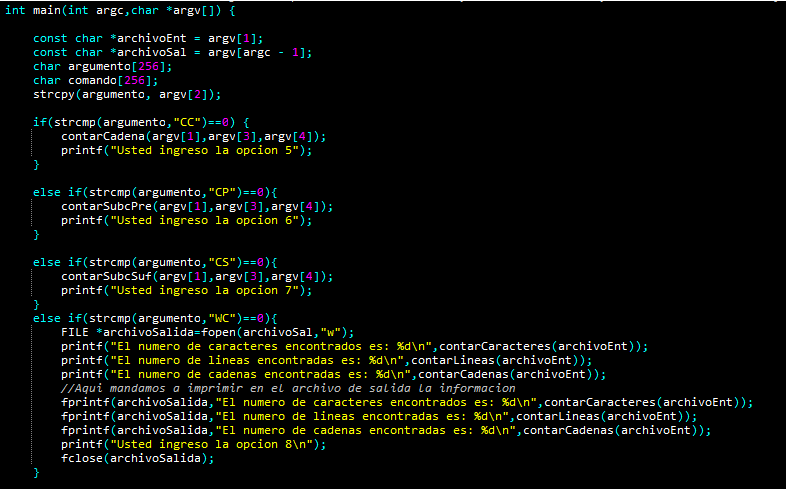
\includegraphics[scale=0.40]{codigo1}\\
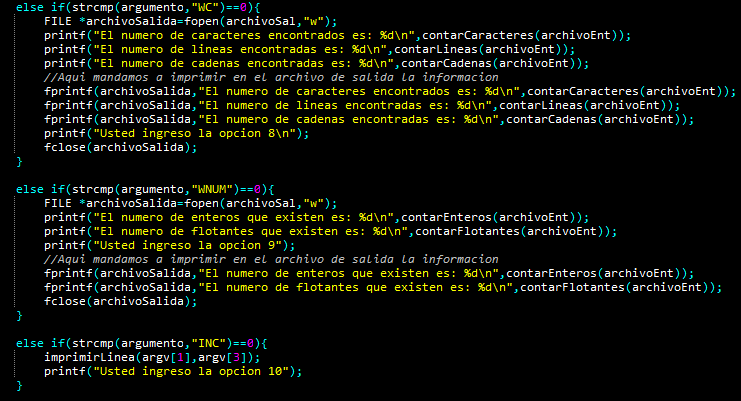
\includegraphics[scale=0.40]{codigo2}
\end{multicols}

Primero, usamos strcpy para copiar el contenido de argv[2] que tiene dentro el comando a utilizar a la variable 'argumento' esto nos permitirá saber que decisión de los if tomar.\\
Aquí es importante señalar que estamos haciendo uso de las anteriores funciones para los puntos 5 al 10 donde tendremos un formato de sintaxis diferente, como se explico anteriormente.\\
Se puede observar que cada decisión tiene dentro una función diferente en ella se encuentran diferentes argumentos en especifico en 4 de las 6 decisiones que fueron mostraron reciben 3 argumentos: \\

\textbf{\textit{ ''ArchivoEntrada.txt''  ''Argumento'' ''ArchivoSalida.txt''}} \\

Que a su vez son;\\

\textbf{\textit{''argv[1]''  ''argv[2]''  ''argv[3]''}}\\

Ahora vamos adentrarnos en cada una de las funciones que se mandan a llamar dentro de cada if y else if

A continuacion se hablara del punto 5 al 7 donde vamos a utlizar la siguente sintaxis, ya mencionada en la pagina 4:\\

\textbf{\textit{ ''argv[0]''  ''argv[1]''  ''argv[2]''  ''argv[3]''  ''argv[4]'' }}\\

Donde la cadena a utilizar sera ''argv[3]''

\newpage
\textbf{\textit{ 5. CC - Contador de Cadenas}}\\

Esta es una funcion de tipo void por lo que la funcion no retornara nada.
\begin{multicols}{2}
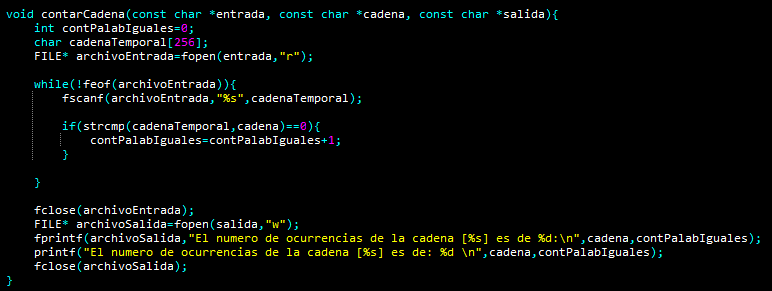
\includegraphics[scale=0.42]{punto5}\\\\
\\Declaramos una función con el nombre ''contarCadenas'' y sera de tipo entero, dentro de ella declaramos dos variables; una sera de tipo int, va actuar como el contador de palabras, la otra de tipo char donde vamos almacenar el contenido del archivo.\\
Abrimos el archivo de entrada que es donde tenemos toda nuestra información guardada, así que vamos a leer su contenido.
\end{multicols}
Después de haber leído el archivo, realizaremos un ciclo donde, mientras que el archivo de entrada no llegue al ''end of file'', extraiga en contenido del archivo, lo guarde en la variable tipo char llamada ''cadenaTemporal'' y mediante una decisión usando la función strcmp de la cual ya hablamos anteriormente, el retorno de la comparación de dos cadenas en este caso la que el usuario escriba y el contenido del archivo, si estas son iguales retornara un 0 y el contador va ir en incremento. Cerramos el archivo de entrada, ahora vamos a abrir el archivo de salida donde vamos a escribir el numero de ocurrencias que tenemos de la palabra indicada por el usuario, asi que mandaremos a imprimir las veces que el contador fue en incremento, al terminar de escribir en el archivo de salida procedemos a cerrar el archivo de salida.\\

\textbf{\textit{ 6. CP - Contador de subcadena prefijos}}\\

Esta es una función de tipo void por lo que la función no retornara nada.
\begin{multicols}{2}
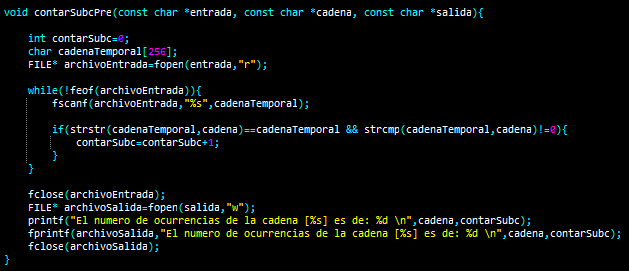
\includegraphics[scale=0.5]{punto6}\\\\
\\Declaramos una función con el nombre ''contarSubPre'' y sera de tipo entero, dentro de ella declaramos dos variables; una de tipo entero y la otra de tipo char, la primera sera un contador, y la ultima para almacenar el contenido del fichero. Abrimos el archivo de entrada para leer su contenido. Ahora realizamos un ciclo donde mientras no sea ''end of file'' almacenaremos el contenido del archivo dentro de la variable char declarada anteriormente, después mediante una condición
\end{multicols}
 ''Si es igual la subcadena de cadena y cadenaTemporal con cadenaTempral y a su vez que el retorno de la comparación entre cadenaTemporal y cadena sea diferente de 0'' esto porque lo que queremos es encontrar el prefijo, que este siempre va a iniciar al principio de cadena, de igual forma consideramos que si queremos saber si perro es prefijo de perro el programa indique que esto es error, ya que el que sean iguales palabras no los hace subcadena de otra. Al cumplir con los parámetros anteriores empezamos a hacer un conteo de palabras que cumplen con el mismo. Cerramos el archivo de entrada y abrimos el archivo de salida que sera el de escritura, mandamos a imprimir en el archivo de salida las veces que el contador aumento mediante un fprintf y por ultimo cerramos el archivo de salida

\textbf{\textit{ 7. CS - Contador de subcadena sufijo}}\\\\
Esta es una función de tipo void por lo que no retornara nada.
\begin{multicols}{2}
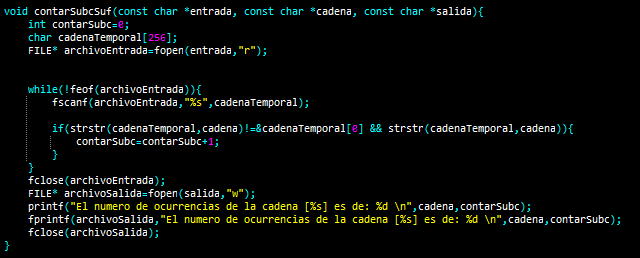
\includegraphics[scale=0.5]{punto7}\\\\
\\Declaramos una función con el nombre ''contarSubSuf'' y sera de tipo entero, dentro de ella declaramos dos variables; una de tipo entero y la otra de tipo char, la primera sera un contador, y la ultima para almacenar el contenido del fichero. Abrimos el archivo de entrada para leer su contenido. Ahora realizamos un ciclo donde mientras no sea ''end of file'' almacenaremos el contenido del archivo dentro de la variable char declarada anteriomente, despues mediante una condicion
\end{multicols}
''Si el retorno de la función strstr() es diferente del apuntador en la primera posición de la variable cadena y si la variable cadena es subcadena de la variable cadenaTemporal''
¿Por qué no queremos que nos retorne el apuntador de la primera posición de la variable cadena? porque no que queremos es encontrar el sufijo por lo que este no se va encontrar en el inicio de la palabra, sera en otra posición de la palabra y a su vez es una subcadena de la otra.\\ Cerramos el archivo de entrada y abrimos el archivo de salida, mandamos a imprimir el valor del contador mediante un fprintf en el archivo de salida y por ultimo cerramos este ultimo.\\

\textbf{\textit{ 8. WC - Contador de cadenas, caracteres y numero de lineas}}\\

\textbf{\textit{\em{Contador numero de lineas}}}
\begin{multicols}{2}

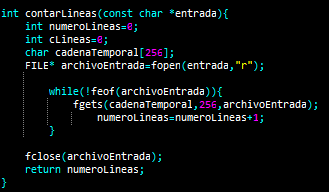
\includegraphics[scale=0.7]{punto8-1}\\
\\Esta es una función de tipo int puesto que retornara un valor al final Declaramos una función con el nombre ''contarLineas'' y sera de tipo entero, dentro de ella declaramos dos variables, una sera el contador de lineas que existen en el archivo de entrada, la otra sera de tipo char, donde almacenara el contenido del archivo. Abrimos el archivo de entrada para lectura, usamos un ciclo while donde 
\end{multicols}
''Mientras no sea ''end of file'' del archivo de entrada'' con un fgets obtendremos el contenido del archivo y lo almacenaremos en la variable cadenaTemporal. Ahora bien, una gran ventaja que tenemos al usar el fgets es que este almacenara linea por linea el contenido de archivo, por lo que al hacerlo, el contador ira en incremento puesto que asi lo tenemos señalado, y cada que realice ese ciclo hasta que se llegue a final del archivo permitirá saber cuantas lineas tenemos.\\
Por ultimo retornamos el numero de conteos que haya realizado el contador.\\
En estas funciones donde tendremos que retornar un valor tendremos que mandarlo a imprimir desde la función main() en su respectivo punto.\\

\newpage
\textbf{\textit{\em{Contador caracteres}}}
\begin{multicols}{2}

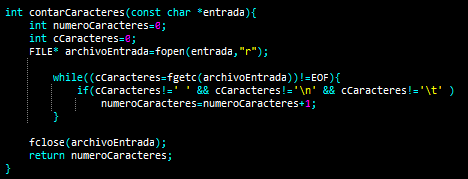
\includegraphics[scale=0.7]{punto8-2}\\
Esta es una función de tipo int puesto que retornara un valor al final.Declaramos una función con el nombre ''contarCaracteres'' y sera de tipo entero, dentro de ella declaramos dos variables, una sera el contador de veces encuentra un carácter en el archivo, la segunda sera de tipo char, donde almacenara el contenido del archivo. Abrimos el archivo de entrada para lectura, usamos un ciclo while donde 
\end{multicols}
''Mientras el valor de cCaracteres (este tendra como contenido carácter por carácter del archivo de entrada) sea diferente del ''end of file'' '' entonces decimos mediante una condición, ''Si cCaracteres es diferente de un espacio vacio y si es diferente de salto de linea (\verb'\'n) y si es diferente de tabulador (\verb'\'t)'' entonces realizara un conteo de los caracteres existentes. Esta condición fue determinada ya que la función fgetc() también toma como el espacio vacio, salto de linea y el tabulador como caracteres, en nuestro caso, nosotros no los tomaremos en cuenta. Por ultimo retornamos el valor del contador.\\

\textbf{\textit{\em{Contador cadenas}}}
\begin{multicols}{2}
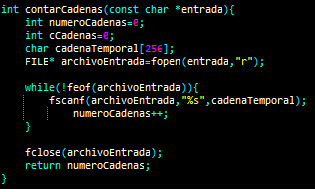
\includegraphics[scale=0.7]{punto8-3}\\
Esta es una función de tipo int puesto que retornara un valor al final.Declaramos una función con el nombre ''contarCadenas'' y sera de tipo entero, dentro de ella declaramos dos variables, una sera el contador de cuantas cadenas existen, la segunda sera de tipo char, donde almacenara el contenido del archivo de entrada. Abrimos el archivo de entrada para lectura, usamos un ciclo while donde 
\end{multicols}
''Mientras no sea ''end of file del archivo de entrada'' vamos a obtener el contenido del archivo y se almacenara en la variable cadenaTemporal, después empezamos a incrementar el contador ¿por que? La función fscanf obtiene solo las palabras, los caracteres de espacio vació y tabuladores no los tomara en en cuenta.
Por ultimo retornamos el valor del contador.\\

\textbf{\textit{\em{Salida}}}
\begin{multicols}{2}

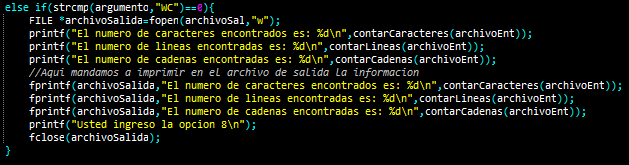
\includegraphics[scale=0.5]{punto8-imprimir}\\\\
\\Aqui se muestra como mandamos a llamar a cada función al main() y su respectivo else if, así mismo, abrimos el archivo de salida donde le indicamos que vamos a escribir sobre el, mandamos a imprimir mediante un fprintf llamamos la función respectiva en este mismo, puesto que retorna un valor.
\end{multicols}

\newpage
\textbf{\textit{ 9. WNUM - Contador de enteros y flotantes}}\\

\textbf{\textit{\em{Contador enteros}}}
\begin{multicols}{2}

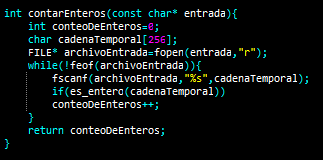
\includegraphics[scale=0.8]{punto9-1}\\\\
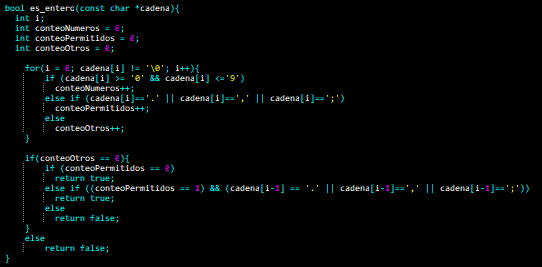
\includegraphics[scale=0.6]{punto9-11}\\

\end{multicols}
Mediante dos funciones una de tipo int y otra boolena donde una retornara un valor entero y la otra retornara un valor boolenano (True o False). 
La funcion de tipo booleano se llamara es \_ entero y se encarga de determinar si un numero encontrado es un entero mediante una serie de condicione, en ella declaramos 4 variables donde todas seran contadores. Un numero entero se caracteriza por: 

\begin{enumerate}
\item No tiene caracteres.
\item No tiene punto (.) y si llegara a tener sera al final del mismo numero de esta forma (9.) con la cual concluimos que es punto final de un texto.
\item No tiene coma (,)  y si llegara a tener sera al final del mismo numero de esta forma (9,) con la cual concluimos que es una pausa del texto.
\item No tiene punto y coma (;)  y si llegara a tener sera al final del mismo numero de esta forma (9;) con la cual concluimos que es una pausa intermedia del texto.

\end{enumerate}
Con una sentencia de control analizaremos cadena por cadena hasta que llegue al final de cadena que es  \verb'\'0 y al reconocer los caracteres que no queremos hará un conteo de ellos, asi mismo llevaremos un conteo de numero que existan en la cadena. Por ultimo mediante los conteo de los caracteres prohibidos diremos si cumple con los aquellos que hacen un numero entero, entonces retorna un valor 'true', de lo contrario 'false'.\\
Ahora con la función int que se llamara contarEnteros declaramos dos variables, una sera el contador de veces que el contador incremento de acuerdo al numero de enteros existentes en el archivo de entrada, la segunda sera de tipo char, donde almacenara el contenido del archivo, obtendremos el contenido del archivo de entrada para después realizar con la función booleana las condiciones para saber si es un entero, por lo que se le pasara la cadena donde guardamos el contenido del archivo.
Abrimos el archivo de entrada para lectura, usamos un ciclo while donde ''mientras no sea ''end of file'' del archivo de entrada'' decimos que si ''se cumple el valor de retorno de la función boolena'' ya que como se menciono la función booleana retornara un valor de true o false dependiendo se si se cumple la función, por lo que si retorna valor de true de acuerdo a las condiciones mencionadas el contador ire en incremento, de lo contrario no incrementara.\\\\

\newpage
\textbf{\textit{\em{Contador flotantes}}}
\begin{multicols}{2}

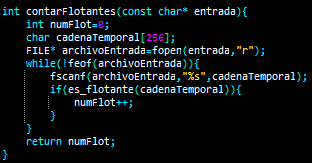
\includegraphics[scale=0.9]{punto9-2}\\\\
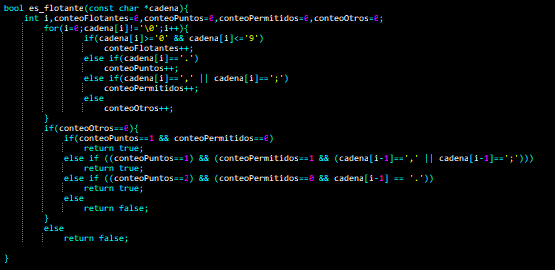
\includegraphics[scale=0.6]{punto9-22}\\

\end{multicols}
Mediante dos funciones una de tipo int y otra boolena donde una retornara un valor entero y la otra retornara un valor boolenano (True o False). 
La función de tipo booleano se llamara es \_ flotante y se encargar de determinar si un numero encontrado es un entero mediante una serie de condiciones en ella declaramos 4 variables donde todas serán contadores. Un numero flotante se caracteriza por: 

\begin{enumerate}
\item No tiene caracteres.
\item Si tiene punto (.) 
\item Si tiene dos puntos, uno tendrá que estar forzosamente al final de este, de esta forma (9.98.) con la cual concluimos que es punto final de un texto.
\item No tiene coma (,)  y si llegara a tener sera al final del mismo numero de esta forma (9.98,) con la cual concluimos que es una pausa del texto.
\item No tiene punto y coma (;)  y si llegara a tener sera al final del mismo numero de esta forma (9.98;) con la cual concluimos que es una pausa intermedia del texto.

\end{enumerate}
Con una sentencia de control analizaremos cadena por cadena hasta que llegue al final de cadena que es \verb'\'0 y al reconocer los caracteres que no queremos hará un conteo de ellos, así mismo llevaremos un conteo de numero que existan en la cadena. Por ultimo mediante los conteo de los caracteres prohibidos diremos si cumple con los aquellos que hacen un numero flotante, entonces retorna un valor 'true', de lo contrario 'false'.
Ahora con la función int que se llamara contarFlotantes declaramos dos variables, una sera el contador de veces que el contador incremento de acuerdo al numero de enteros existentes en el archivo de entrada, la segunda sera de tipo char, donde almacenara el contenido del archivo, obtendremos el contenido del archivo de entrada para después realizar con la función booleana las condiciones para saber si es un entero, por lo que se le pasara la cadena donde guardamos el contenido del archivo.
Abrimos el archivo de entrada para lectura, usamos un ciclo while donde ''mientras no sea ''end of file'' del archivo de entrada'' decimos que si ''se cumple el valor de retorno de la función boolena'' ya que como se menciono la función booleana retornara un valor de true o false dependiendo se si se cumple la funcion, por lo que si retorna valor de true de acuerdo a las condiciones mencionadas el contador ire en incremento, de lo contrario no incrementara.\\

\newpage

\textbf{\textit{\em{Salida}}}
\begin{multicols}{2}

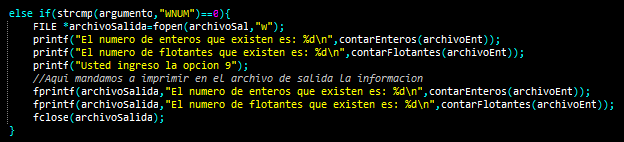
\includegraphics[scale=0.5]{punto9-imprimir}\\\\
Ahora mandamos a llamar las funciones de tipo int donde las vamos a andar a imprimir mediante un fprintf puesto que estas retornan un valor.
\end{multicols}

\textbf{\textit{ 10. INC - Imprimir lineas de un archivo con su numero de linea.}}\\

Esta es una función de tipo void por lo que la funcion no retornara nada.
\begin{multicols}{2}
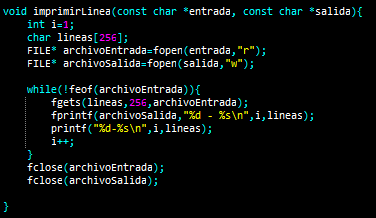
\includegraphics[scale=0.7]{punto10}\\\\
Declaramos una función con el nombre ''imprimirLineas'' y sera de tipo entero, dentro de ella declaramos dos variable; una sera de tipo int y llevara el conteo de numero de linea, la otra sera de tipo char, almacenara el contenido del archivo. Abrimos el archivo de entrada y abrimos el archivo de salida; en el primero es lectura, el ultimo escribiremos lo requerido. 
\end{multicols}
Con un ciclo while decimos que ''mientras no sea ''end of file'' del archivo de entrada'' entonces obtenemos el contenido del archivo linea por linea con fgets y lo almacenaremos en la variable declarada anteriormente. Mandamos a imprimir cada linea y realizamos un conteo hasta que lleguemos al final del archivo. Por ultimo cerramos el archivo de entrada y salida.

\newpage
\textbf{\textit{ Manejo de los primeros 4 puntos.}}\\

Ahora hablaremos de los puntos 1 al 4 donde en la parte anterior se saltaron, puesto que esta es la estructura que sigue el programa. A continuación de explicara el porque.\\
De acuerdo a los requerimientos del programa, del punto 1 al 4 pide ingresar un argumento seguido de un guion bajo y un numero, de acuerdo a la preferencia del usuario, por ejemplo, esta seria un argumento referente al punto 1 L\_ 1\_2 \_3, significa que el usuario eligió la opcion 1 que es L, reconoceremos los caracteres que estan antes del primer guion bajo como ''Comando'' y desea manejar las lineas 1, 2 y 3 del archivo de enterada.\\
Para identificar el comando y realice una determinada acción haremos uso de sscanf donde vamos extraer del argumento que va escribir el usuario el comando con '' \%[ \verb'^'\_] '' decimos que solo obtenga todo lo que este antes del primer \_ donde se almacenara en la variable ''comando''. asi mismo vamos a obtener lo que sigue hacia la derecha del primer \_ donde eso lo vamos a almacenar en la misma variable ''argumento'', por lo que al final de la función sscanf el valor de argumento \\

\begin{multicols}{2}

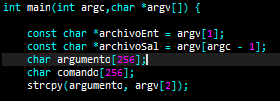
\includegraphics[scale=0.9]{variablesint}
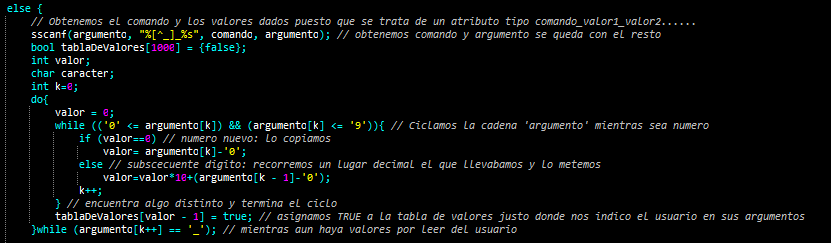
\includegraphics[scale=0.5]{obtArgCom}

\end{multicols}
En la imagen de la izquierda tenemos las variables del int main() y son:
char *archivoEnt = argv[1], char *archivoSal = argv[argc - 1], char argumento[256], char comando[256];
Las dos primeras variables que son punteros serán para representar los archivos de entrada y salida, las ultimas dos serán para reconocer argumento y comando como ya lo mencionamos anteriormente, así que almacenaran su contenido. De primeras diremos que argumento sera lo escrito por el usuario, así que se copia el contenido de 'argv[2]' a la variable 'argumento'.\\
En la imagen de la derecha es el código con el que obtendremos el argumento y comando así mismo empezamos el desarrollo de los 4 puntos faltantes. Comenzamos con las variables a utilizar y serán 4; bool tablaDeValores[1000] = {false}, int valor, char carácter, int k=0. El propósito de la variable bool es para construir una tabla con valores false, 'valor' sera un contador que va recorrer dicha tabla y 'k' también actuara como un contador que va a recorrer la cadena original. \\
Así que mediante un ciclo do-while vamos a recorrer el ultimo valor que le dimos a la variable ''argumento'', recordemos que tiene almacenado del primer \_ hacia la derecha. Al recorrer argumento mediante ciclos y sean números los que vaya encontrado los almacenara en la variable 'valor' por medio de una resta de ascii, y si el numero llegara a ser de dos dígitos este hará una operación donde permita corvertirlo a un numero de dos digitos.\\
Ahora ese valor que vaya tomando la variable valor lo ira almacenando en la tabla de valores, donde le diremos que en, la casilla donde nosotros tenemos como valor le asigne el valor de 'true' de esta forma podremos manipular cuando el usuario indique un cierto numero de linea, parrafo etc.

\newpage
\textbf{\textit{ 1. L\_  Imprimir lineas indicadas}}\\
\begin{multicols}{2}

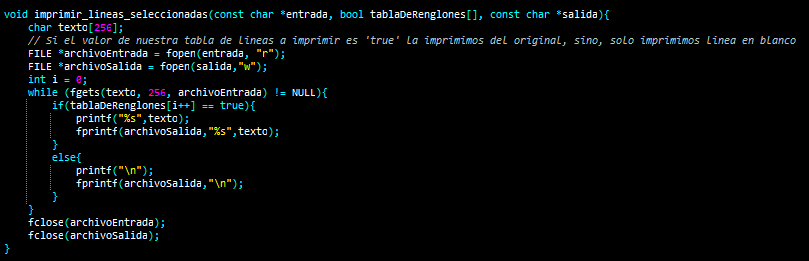
\includegraphics[scale=0.4]{punto1}
Declaramos una función de tipo void llamada 'imprimir\_ lineas\_ seleccionadas' donde no vamos a retornar nada, dentro de ella declaramos dos variables una de tipo char; almacenaremos el contenido del archivo en ella y la otra de tipo int que sera encargada de ser contador.\\
Abriremos los archivos de entrada y salida, uno sera de lectura y el otro sera donde escribiremos.\\
\end{multicols}
Ahora diremos que ''mientras que sea diferente de null el obtener el contenido de el archivo en la variable texto'' observemos que haremos uso de fgets donde obtendremos linea por linea mientras se realice el ciclo. procedemos a decir que ''si en la tabla de valores (esta se ira recorriendo por el contador) existe el valor de verdad, que en ese numero de linea la imprima en el archivo de salida, de no ser asi no imprimirá nada y solo serán saltos de linea.\\ 
Por ultimo cerramos los dos archivos.\\

\textbf{\textit{ 2. C\_  Imprimir columnas indicadas}}\\

\begin{multicols}{2}
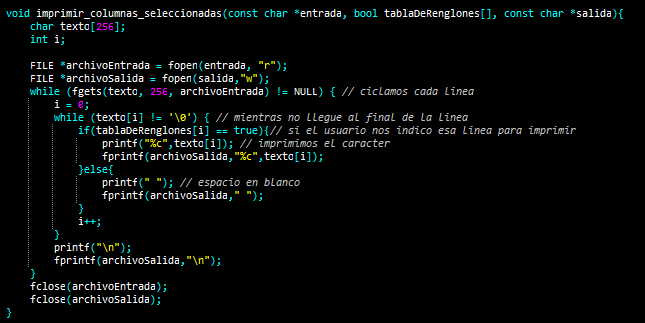
\includegraphics[scale=0.5]{punto2}
Declaramos una función de tipo void llamada 'imprimir\_ columnas\_ seleccionadas' donde no vamos a retornar nada, dentro de ella declaramos dos variables una de tipo char; almacenaremos el contenido del archivo en ella y la otra de tipo int que sera encargada de ser contador.\\
Abriremos los archivos de entrada y salida, uno sera de lectura y el otro sera donde escribiremos.\\
\end{multicols}

Ahora diremos que ''mientras que sea diferente de null el obtener el contenido de el archivo en la variable texto'' observemos que haremos uso de fgets donde obtendremos linea por linea mientras se realice el ciclo, utilizaremos otro ciclo while para recorrer cada cadena y ''mientras no llegue a final de cadena'' ''si en la tabla de valores (esta se ira recorriendo por el contador) existe el valor de verdad, que en ese caracter lo imprima en el archivo de salida, de no ser asi no imprimira nada\\
Por ultimo cerramos los dos archivos.\\


\textbf{\textit{ 3. ILV\_  Imprimir salto de lineas en las lineas indicadas}}\\
\begin{multicols}{2}

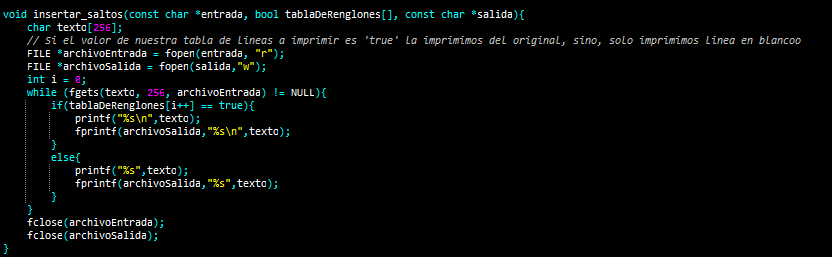
\includegraphics[scale=0.4]{punto3}
Declaramos una función de tipo void llamada 'insertar\_ saltos' donde no vamos a retornar nada, dentro de ella declaramos dos variables una de tipo char; almacenaremos el contenido del archivo en ella y la otra de tipo int que sera encargada de ser contador.\\
Abriremos los archivos de entrada y salida, uno sera de lectura y el otro sera donde escribiremos.\\
\end{multicols}
Ahora diremos que ''mientras que sea diferente de null el obtener el contenido de el archivo en la variable texto'' observemos que haremos uso de fgets donde obtendremos linea por linea mientras se realice el ciclo. Procedemos a decir que ''si en la tabla de valores (esta se ira recorriendo por el contador) existe el valor de verdad, que en ese numero de linea la imprima junto con un salto de linea en el archivo de salida, de no ser asi, solo imprimirá las lineas sin alto de linea.\\ 
Por ultimo cerramos los dos archivos.\\

\textbf{\textit{ 4. IC\_  Imprimir tabulador en las columnas indicadas}}\\
\begin{multicols}{2}

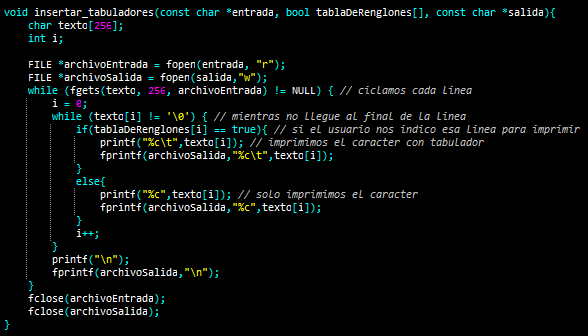
\includegraphics[scale=0.5]{punto4}\\
Declaramos una función de tipo void llamada 'insertar\_ tabulador' donde no vamos a retornar nada, dentro de ella declaramos dos variables una de tipo char; almacenaremos el contenido del archivo en ella y la otra de tipo int que sera encargada de ser contador.\\
Abriremos los archivos de entrada y salida, uno sera de lectura y el otro sera donde escribiremos.\\
\end{multicols}
Ahora diremos que ''mientras que sea diferente de null el obtener el contenido de el archivo en la variable texto'' observemos que haremos uso de fgets donde obtendremos linea por linea mientras se realice el ciclo. Procedemos a decir que ''si en la tabla de valores (esta se ira recorriendo por el contador) existe el valor de verdad, que en ese numero de carácter con un tabulador la imprima en el archivo de salida, de no ser así no imprimirá los demás caracteres de manera normal\\ 
Por ultimo cerramos los dos archivos.
\end{document}
